\section{Теоритические сведения}
\subsection{Распространение плоских монохроматических волн в одноосных кристаллах}
В некоторых кристаллах потенциальные ямы, в которых находятся электроны вблизи узлов решетки, не являются сферически симметричными. Для малых отклонений от положения равновесия потенциальная энергия электрона будет иметь вид
\[
    U  = a_{x}x^{2} + a_{y}y^{2} + q_{z}z^{2}
\]
Если $a_{y} = a_{z} = a_{\perp}$, $a_{x} = a_{\parallel}$, то кристалл называется одноосным с оптической осью $x$.

Так как одноосный кристалл неизотропен, векторы $\vec{E}$ и $\vec{D}$ в общем случае неколлинеарны:
\[
\vec{D} = \varepsilon_{\perp}\vec{E}_{\perp} + \varepsilon_{\parallel}\vec{E}_{\parallel}
\]

Распространение электромагнитных волн в отсутствие электрических зарядов и токов описывается уравнениями
\[
    \rot \vec{H} = \frac{1}{c}\frac{\partial \vec{D}}{\partial t}
\]
\[
    \rot \vec{E} = -\frac{1}{c}\frac{\partial\vec{H}}{\partial t}
\]
Плоские монохроматические волны в таких условиях описываются уравнениями
\[
    \vec{E} = \vec{E_{0}}\exp{\left(i\left(\omega t - \vec{k}\vec{r}\right)\right)}
\]
\[
    \vec{H} = \vec{H_{0}}\exp{\left(i\left(\omega t - \vec{k}\vec{r}\right)\right)}
\]
\[
    \vec{D} = \vec{D_{0}}\exp{\left(i\left(\omega t - \vec{k}\vec{r}\right)\right)}
\]
Отсюда следует, что $\rot\vec{H} = -i\vec{k}\times\vec{H}$, $\frac{\partial \vec{D}}{\partial t} = i \omega \vec{D}$ и аналогичные выражения для других векторов.

Подставив эти значения в уравнения Максвелла, получаем
\[
    \vec{D} = -\frac{c}{ \omega} \vec{k} \times \vec{H}
\]
\[
    \vec{H} = \frac{c}{ \omega} \vec{k} \times \vec{E}
\]

Отсюда видно, что $\vec{D}$, $\vec{H}$ и $\vec{k}$ взаимно перпендикулярны, а $\vec{E}$ лежит в одной плоскости с $\vec{D}$ и $\vec{k}$.

\begin{figure}[ht!]
    \center{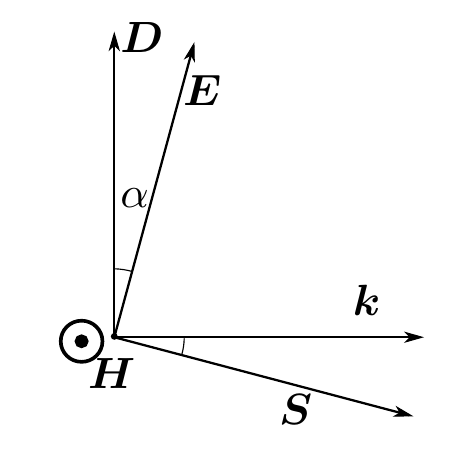
\includegraphics[width=0.4\linewidth]{../img/dehsk.png}}
\end{figure}

При этом выполнение материалистического уравнения возможно только если $\vec{D}$ перпендикулярен плоскости, в которой лежат оптическая ось кристалла и $\vec{k}$ (обыкновенная волна, рисунок слева), либо лежит в ней (необыкновенная волна, рисунок справа).

\begin{figure}[ht!]
    \center{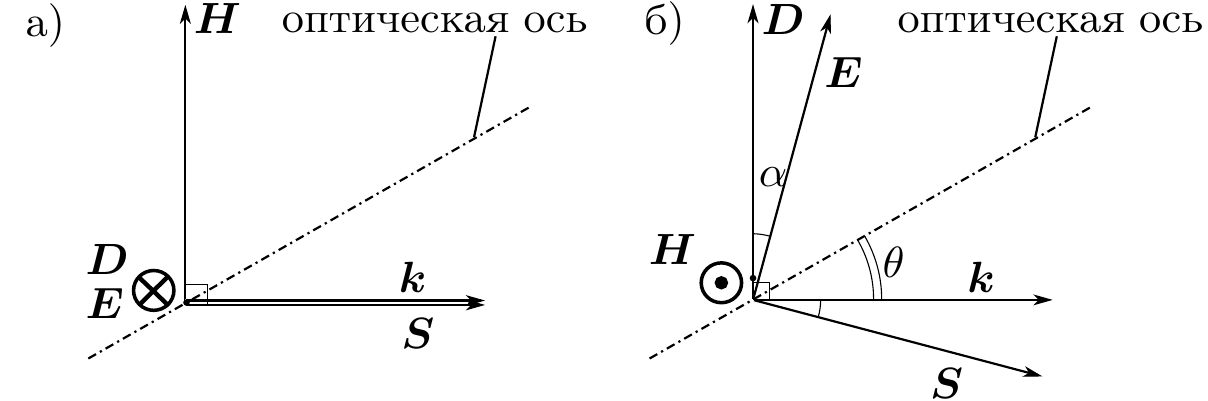
\includegraphics[width=0.8\linewidth]{../img/the.png}}
\end{figure}

Обыкновенная и необыкновенная волны распространяются в кристалле с разной скоростью. Обыкновенная волна поперечна относительно $\vec{E}$ и $\vec{H}$, поэтому для нее уравнения Максвелла те же, что и в изотропных средах, а скорость распространения
\[
    v_{\text{о}} = \frac{c}{\sqrt{ \varepsilon_{\perp}}} = \frac{c}{n_{\text{о}}}
\]
$n_{\text{о}} = \sqrt{ \varepsilon_{\perp}}$~--- коэффициент преломления обыкновенной волны.

Найдем фазовую скорость необыкновенной волны.
\[
    v = \frac{ \omega}{k} = \frac{cH}{D} = \frac{cE\cos \alpha}{H}, \text{См. рисунок и формулы связи $\vec{D}$, $\vec{E}$, $\vec{H}$ и $\vec{k}$}
\]
Исключая $H$ и выражая угол $ \alpha$ через скалярное произведение, получим
\[
    v = c\sqrt{\frac{E \cos \alpha}{D}} = c\sqrt{\frac{\vec{E} \vec{D}}{D^{2}}}
\]
\[
    \vec{E} \vec{D} = \varepsilon_{\parallel}E^{2}_{\parallel} + \varepsilon_{\perp}E^{2}_{\perp} = \frac{D_{\parallel}^{2}}{ \varepsilon_{\parallel}} + \frac{D_{\perp}^{2}}{ \varepsilon_{\perp}} = D^{2} \left(\frac{\sin^{2} \theta}{\varepsilon_{\parallel}} + \frac{\cos^{2} \theta}{ \varepsilon_{\perp}}\right)
\]

Получаем:
\[
    v_{\text{e}} = \frac{c}{n( \theta)}
\]
\[
n(\theta) = \frac{1}{\sqrt{\frac{\sin^{2} \theta}{ \varepsilon_{\parallel}} + \frac{\cos^{2} \theta}{ \varepsilon_{\perp}}}}
\]

Фазовая скорость необыкновенной волны зависит от угла между оптической осью и волновым вектором. Кроме того, вектор Поинтинга не коллинеарен волновому вектору, поэтому направление переноса энергии и переноса фазы не совпадают.

Плоская монохроматическая волна, попадающая из изотропной среды в одноосный кристалл, распадается на две взаимно ортогональные плоские волны, которые распространяются в разных направлениях и с разными скоростями.

\begin{figure}[ht!]
    \center{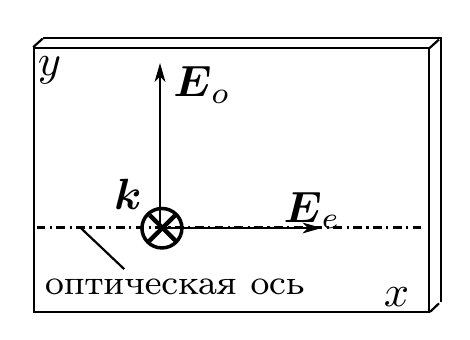
\includegraphics[width=0.4\linewidth]{../img/plast.png}}
\end{figure}
Важным частным случаем является распространение волн в одноосном кристалле перпендикулярно оптической оси. При этом у обыкновенной оси вектор $\vec{E}$ колеблется в плоскости, перпендикулярной этой оси. Для обыкновенной волны показатель преломления $n_{o} = \sqrt{ \varepsilon_{\perp}}$, а для необыкновенной $n_{e} = \sqrt{ \varepsilon_{\parallel}}$ (т.к. $ \theta = 90^{\circ}$).

Для нормально падающей волны компоненты обыкновенной и необыкновенной волн будут распространяться независимо и к моменту выхода наберут разность фаз
\[
    \Delta \varphi = kh\left(n_{e} - n_{o}\right)
\]

\subsection{Интерференция на одноосном кристалле}

Если перед одноосным кристаллом, помещенным между скрещенными поляроидами, поместить матовую пластинку, после которой лучи будут рассеиваться под разными углами, то на выходе образуется интерференционная картина в виде концентрических окружностей, перерезанных крестом. Эту картину образовали обыкновенные и необыкновенные лучи.

Коэффициент преломления для обыкновенного луча не зависит от угла падения на пластинку и равен $n_{1} = n_{o}$. Для необыкновенного луча в приближении малых углов $n_{2} = n_{o} - \left(n_{o} - n_{e}\right) \theta^{2}$. Таким образом разность фаз составляет
\[
    \Delta \varphi = \frac{2 \pi}{ \lambda} l \left(n_{o} - n_{e}\right) \theta^{2}
\]

Направлениями постояной разности фаз служат конусы. Из-за этого картина предствляет собой концентрические окружности. Крест выделяет те области, в которых распространяется только одна волна (обыкновенная или необыкновенная). При повороте выходного поляроида на $90^{\circ}$ картина меняется на противоположную.

Найдем радиус темного кольца $m$ в случае скрещенных поляроидов. При $m = 0$ сдвиг фаз равен нулю и луч не проходит анализатор. При сдвиге фаз $2\pi m$ ситуация аналогична. Поэтому
\[
    2\pi m = \frac{2\pi}{\lambda} l \left(n_{o} - n_{e}\right) \theta^{2}
\]
$\theta_{\text{внешн}} = n_{o}\theta$, поэтому
\[
    r_{m}^{2} = \frac{\lambda}{l} \frac{\left(n_{o}L\right)^{2}}{\left(n_{o} - n_{e}\right)} m
\]

\subsection{Влияние электрического поля}
Изотропное вещество можно превратить в неизотропное, поместив его в сильное электрическое поле. В этом случае электроны смещаются к новому положению равновесия и в потенциальной энергии появляются составляющие высоких порядков:
\[
    U = ax^{2} + \beta x^{3} + \gamma x^{4}
\]

Если $\beta \ne 0$, то вторая производная энергии окажется линейной функцией и получится эффект Поккельса: появится наведенное двулучепреломление, разность показателей преломления которого пропорциональна приложенному напряжению.

\begin{figure}[ht!]
    \center{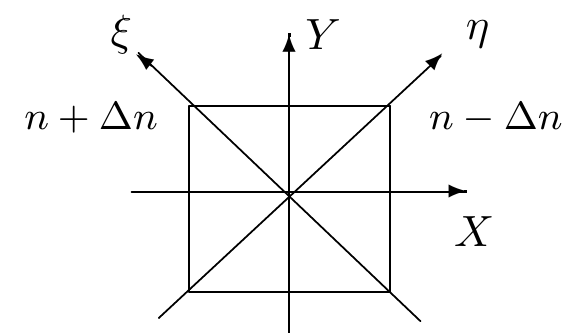
\includegraphics[width=0.5\linewidth]{../img/pok.png}}
\end{figure}

Поместим одноосный кристалл с осью $z$ в электрическое поле $E_{\text{эл}}$, направленное вдоль $x$. В данной работе свойства кристалла таковы, что в плоскости $xy$ появятся дополнительные перпендикулярные направления под углами $45^{\circ}$ к осям $x$ и $y$ с показателями преломления $n_{o} + \Delta n$ и $n_{o} + \Delta n$. Причем $\Delta n = A E_{\text{эл}}$. 

Пусть свет на входе в кристалл поляризован вертикально, а анализатор пропускает горизонтальную поляризацию. Разложим исходный вектор $E = E_{0} exp{\left(i\left(\omega t - kz\right)\right)}$ по осям $\xi$ и $\eta$. $E_{\xi} = E_{\eta} = E_{0} / \sqrt{2}$. После прохождения кристалла между векторами $E_{\xi}$ и $E_{\eta}$ появится разность фаз
\[
    \Delta \varphi = \frac{4\pi l}{\lambda}AE_{\text{эл}} = \frac{4\pi}{\lambda}\frac{l}{d}AU
\]
$U$~--- напряжение на кристалле, $d$~--- его поперечный размер.

Результирующее поле после анализатора~--- сумма проекций $E_{\xi}$ и $E_{\eta}$ на $x$:
\[
    E_{\text{вых}} = \frac{E_{0}}{2}\exp{\left(i\left(\omega t - kl\right)\right)}\left(e^{i\Delta \varphi / 2} - e^{-i\Delta\varphi / 2}\right) = E_{0}\exp{\left(i\left(\omega t - kr\right)\right)} \sin \left(\frac{ \Delta \varphi}{2}\right)
\]
В случае параллельных поляризаторов
\[
    E_{\text{вых}} =E_{0}\exp{\left(i\left(\omega t - kr\right)\right)} \cos \left(\frac{ \Delta \varphi}{2}\right) 
\]
Интенсивность света пропорциональна квадрату $E$. В случае скрещенных поляроидов:
\[
    I_{\text{вых}} = I_{0} \sin^{2} \left(\frac{ \Delta \varphi}{2}\right) = I_{0} \sin^{2} \left(\frac{\pi}{2}\frac{U}{U_{\lambda / 2}}\right) 
\]
В случае параллельных
\[
    I_{\text{вых}} = I_{0} \cos^{2} \left(\frac{\pi}{2}\frac{U}{U_{\lambda / 2}}\right)
\]

\[
    U_{\lambda /  2} = \frac{\lambda}{4A}\frac{d}{l}
\]
~--- полуволновое напряжение. При $U=U_{\lambda / 2}$ сдвиг фаз между двумя волнами равен $\pi$. 

